\section{Interpretations}
\label{sec:interpretations}
As a demonstration of how the data may be re-interpreted, two well-motivated BSM scenarios are selected and the unfolded measurements of Section~\ref{sec:m4lresults} are used to set exclusion limits on the parameter space of both. The first considers the Standard Model in an effective field theory (EFT) framework, and the second is a gauged B-L model that introduces a heavy Higgs and a new gauge boson. The EFT limits are presented in this section, while the $B-L$ limits are presented in Section~\ref{ssec:BL:ATLAS} of Chapter~\ref{chap:reinterpretation}, in conjunction with limits set by the \contur reinterpretation tool. Note that the author did not explicitly work on the interpretation studies within the analysis - all results are credited to relevant members of the analysis team. This section is discussed in detail due to its relevance to the re-interpretation theme.

Each model has multiple variants which differ in value for some adjustable parameter. This could be, for example, the mass of a new particle or the strength of a new coupling constant These variants can be compared as explanations for the same observed data, and the probability of the variant being true can be calculated. This probability to obtain the exact data observations given the parameters at is known as the likelihood of that variant of the model. The maximum likelihood (ML) estimate is defined as the parameter value at which the likelihood at a maximum. Accordingly, a maximum likelihood estimator (MLE) returns the value of the parameter which, given the data, is most likely. 

A likelihood function is constructed using only the published results of the measurement and is used to set limits on the BSM models. It has the form
\begin{equation}\label{eq:likelihood}
    \mathcal{L} = \frac{1}{\sqrt{ \left(2\pi\right)^k | C |}} \exp \left( - \frac{1}{2} \left( \sigdata - \sigpred(\vec{\theta}) \right)^T C^{-1} \left(  \sigdata - \sigpred(\vec{\theta})  \right) \right) \times \prod_{i} \mathcal{G}\left(\theta_{i}, 0, 1\right),
\end{equation}
where $C$ is the measurement covariance matrix, and \sigdata and \sigpred $k$-dimensional vectors of the measured and predicted cross-sections respectively. The uncertainties in the BSM prediction are included as Gaussian constrained nuisance parameters $\theta$; meaning the uncertainties come from imperfect knowledge of the model parameters. This approach to calculate the likelihood is much less computationally expensive than an extensive Gaussian model. The total covariance matrix is $C$ is the sum of the statistical and systematics uncertainty matrices and the Standard Model theory uncertainty matrix. For the statistical uncertainty, the predicted uncertainty from the expected Standard Model yield is used instead of what is observed in data. This was the result of a study which showed that the data's downward fluctuations in bins with lower statistics resulted in a biased best fit value as well as non-optimal intervals, and a non-asymptotic test statistic~\cite{m4l_internalnote}. 

For any given point in the BSM parameter space, there may be different effects on various distributions. In order to obtain the most stringent limit, it is necessary to examine the effect on each of the unfolded kinematic observable present in section \ref{sec:m4lresults}. There are a total of twelve observables - those that are measured in slices of another count as one observable with the slices combined. Due to the lack of statistical correlation between the observables, the one providing the best expected sensitivity is used to set the limit \cite{m4l2021_paper}.

\subsection{\ZFourL branching fraction}
The measured cross-section in the single $Z$ region from table \ref{tab:fidxs} is used to extract the single resonant \ZFourL decay branching fraction and the result is compared to previous LHC measurements. For ease of comparison, phase space corrections are applied the branching fraction so it matches that of previous analyses. 

First, the predicted contribution from sources other than \qqFourL{} ($\sigma_{\text{non-}qq\to 4\ell}^{\text{pred}}=0.22\pm0.04$) are subtracted from the measured cross-section ($\sigma_{\text{meas}}$) in the \ZFourL enriched region. Next, contributions originating from $t-$channel $ZZ$ production rather than single $Z$ production are accounted for with $f_{Z}=0.952\pm0.005$. A tau correction factor of $f_{\tau}=0.99186\pm0.00014$ is also applied; this is the fraction of events where no leptons originate from tau decays. In the denominator, $\sigma_Z$ is the total production cross-section for single $Z$ as quoted in the \ATLAS measurement of Reference~\cite{ATLAS_WZXS}. Finally, the fiducial correction factor $A_{\text{fid}}0.935 \pm 0.001$ accounts for the difference in the Z mass window definition. This calculation is written as
\begin{equation*}
    \mathcal{B}_{Z\rightarrow 4\ell} = \frac{\left(\sigma^{\text{meas}}-\sigma_{\text{non-}qq\to 4\ell}^{\text{pred}}\right) \times f_{\text{non-}\tau} \times (1-f_{\text{qqZZ, non-res}})}{\sigma_{Z} \times A_{\text{fid}}},
\end{equation*}
where 
\begin{equation*}
    \sigma_{\text{unfolded}} = \left(22.1 \pm 0.7(\text{stat}) \pm 1.1(\text{sys}) \pm 0.4 (\text{lumi})  \right)\text{fb} 
\end{equation*}
is the unfolded cross-section in the single $Z$ region (see Section~\ref{sec:m4lresults}) and  
\begin{equation*}
    \sigma_{\text{pred, non-qqZZ}} =  \left(0.222 \pm 0.036(\text{sys}) \pm 0.001 (\text{stat}) \pm 0.004 (\text{lumi}))\text{fb} = (0.22\pm 0.04 \right) \text{fb}
\end{equation*}
is the predicted contribution in the same region from sources other than $qq\to ZZ$. It is estimated using the respective theoretical predictions at particle-level. 

The resulting \ZFourL branching fraction is measured to be
\begin{align*}
    \mathcal{B}_{Z\rightarrow 4\ell} & = \left( 4.41 \pm 0.13 \left[\text{stat}\right] \pm 0.23 \left[\text{exp. sys}\right] \pm 0.09 \left[\text{theory}\right]\pm 0.12 \left[\text{lumi}\right] \right) \times 10^{-6} \\
    & =  \left( 4.41 \pm 0.30 \right) \times 10^{-6}
\end{align*}
with the quoted statistical, systematic, theoretical, luminosity, and combined uncertainties. This result is compatible with the previous measurements from \CMS and \ATLAS~\cite{Aaboud:2019lxo,Sirunyan:s10052-018-5567-9,Aaboud:2014zbr}, and is the highest precision measurement of the \ZFourL branching fraction achieved at the \LHC to date. 

\subsection{EFT couplings}

A simple example of an effective field theory (EFT) is the Fermi theory of beta decay. In this theory postulated in 1933, the neutron decay occurs in a point-like manner to an electron, a proton, and a neutrino. In the underlying model (the SM), the "point" is characterized by the emission of a \W boson by a down quark which then transforms into an up quark. The \W boson decays to an electron and a neutrino. The Fermi theory effective Lagrangian describing this interaction contains $G_{\text{F}}$, the Fermi constant. $G_{\text{F}}$ is proportional to the ratio of the weak coupling constant to the mass of the \W boson. This was only discovered later on, however, and at the time knowing only the Fermi constant was a sufficient way to model the process. The \W boson has a mass that is an order of magnitude higher than the typical energy of $\beta$ decays, and has been integrated out in the Fermi theory. This is said to be an effective field theory calculation, which is consistent way to describe a higher-order process so long as the energy scale $E$ of the process is small compared to the energy scale $\Lambda$ of the mediating heavy state \cite{De_Simone_2016}. The scale hierarchy $E \ll \Lambda$ is a fundamental property of an EFT \cite{Brehmer2016}.

The Standard Model in the Effective Field Theory approach, often abbreviated as SMEFT, is an expansion of the Standard Model Lagrangian that introduces higher dimension operators suppressed by powers of $\Lambda$. The suppression increases by $\Lambda^1$ for each successive increase in dimension. $\Lambda$ represents the mass scale of BSM particles, and for the EFT to hold its validity the processes probed should be lower than $\Lambda$. The theory is required to contain the Standard Model gauge groups, and at low energies it must reduce to the Standard Model. The Standard Model Lagrangian contains operators of dimension-four, so the expansion for the SMEFT Lagrangian starts at dimension-five and is written as
\begin{equation}
    \lagrangian_{\text{SMEFT}}=\lagrangian_{\text{SM}} + \sum_{i}\dfrac{c_i^5}{\Lambda^{}}\mathcal{O}_i^5 + \sum_{i}\dfrac{c_i^6}{\Lambda^{2}}\mathcal{O}_i^6 + \sum_{i}\dfrac{c_i^7}{\Lambda^{3}}\mathcal{O}_i^7 + 
    \sum_{i}\dfrac{c_i^8}{\Lambda^{4}}\mathcal{O}_i^8 +\cdots
\end{equation}
where $\Lambda$ is the energy scale at which new physics appears, $\mathcal{O}_i^d$ are operators of dimension-$d$, and $c_i^d$ are the coupling constants for the operators, also called the Wilson coefficients. 

For each dimension, a complete set of operators must be computed for the expansion. Starting with dimension-five operators, S. Weinberg showed in reference \cite{Weinberg_1979} that it violates lepton number. Some decades later, reference \cite{de_Gouv_a_2014} demonstrated that there are no \SMgroup gauge-invariant odd-dimentional operators that preserve both baryon and lepton number \cite{Kobach_2016}. Higher even dimensions are very suppressed by factors of $\Lambda$. It is for these reasons that in the SMEFT framework considered for the four lepton analysis only dimension-six operators are considered. The effective Lagrangian is therefore defined as 
\begin{equation} \label{eq:SMEFTdim6lagragian}
    \lagrangian_{\text{SMEFT}}=\lagrangian_{\text{SM}} + \sum_{i}\dfrac{C_i^6}{\Lambda^{2}}\mathcal{O}_i^6.
\end{equation}
A common notation is to absorb the $\Lambda^2$ into the Wilson coefficient, thus redefining them as $c_i=\frac{C_i}{\Lambda^2}$. A complete and non-redundant basis for the fifty-nine independent dimension-six operators can be found in reference \cite{Grzadkowski_2010}.

% http://cds.cern.ch/record/2699893/files/CERN-THESIS-2019-205.pdf

Following the Lagrangian of equation \ref{eq:SMEFTdim6lagragian}, the amplitude is computed as
\begin{equation}
\mathcal M_{Mix} = \mathcal M_{SM} + c_i \mathcal M_{\text{EFT, }d=6}
\end{equation}
where $c_i$ represent any Wilson coefficient. The matrix element squared reads
\begin{equation}\label{eq:EFTamplitude}
 \left | \mathcal  M_{Mix} \right |^2  = 
\left |  \mathcal M_{SM} \right |^2 +
c_i 2 \mathcal R \left ( M_{SM}^{*} M_{\text{EFT, }d=6} \right) +
c_i^2  \left |  \mathcal M_{\text{EFT, }d=6} \right |^2. 
\end{equation}
Here the first term represents the Standard Model contribution, the third term is the pure BSM component, and the second term describes the interference effect between the Standard Model and the effective field theory. 

If the effective field theory framework is assessed in context of dimension-six and higher dimension operators, the square of the matrix element is written as 
\begin{equation}
  \begin{aligned}
  \left|\mathcal M\right|^2 =& \left| \mathcal M_{SM} + \frac{C_{i,6}}{\Lambda^{2}} \mathcal M_{\text{EFT, dim6},i}  + \frac{C_{i,8}}{\Lambda^{4}} \mathcal M_{\text{EFT, dim8},i} + \ldots \right|^2 \\
  \left|\mathcal M\right|^2 =& \underbrace{\left|\mathcal M_{SM}\right|^2}_{\mathcal{O}(1)} +  
  \underbrace{2 \frac{C_{i,6}}{\Lambda^{2}} \mathcal{R} \left(\mathcal M_{\text{EFT, dim6},i}^{\ast} \mathcal M_{SM} \right)}_{\mathcal{O}(\Lambda^{-2})}   \\ 
  &  + \underbrace{
      \frac{C_{i,6}^2}{\Lambda^{4}} \left| \mathcal M_{\text{EFT, dim6},i} \right|^2
      + 2 \frac{C_{i,8}}{\Lambda^{4}} \mathcal{R} \left(\mathcal M_{\text{EFT, dim8},i}^{\ast} \mathcal M_{SM} \right)
    }_{\mathcal{O}(\Lambda^{-4})} +  \ldots . 
  \end{aligned}
\end{equation}
The Wilson coefficients here are written in their raw form with the exponential of $\Lambda$ included in the denominator. It is interesting to note that the quadratic term of the dimension-six operators are suppressed by the same $\Lambda^{-4}$ as the interference term of the dimension-eight operators with the Standard Model contribution. This motivates the construction of a linear-only model alongside the full model, where terms higher than order $\Lambda^{-2}$ are ignored. For the dimension-six model, the linear-only limit sets the third term of equation \ref{eq:SMEFTXS} to zero. 

Considering the resulting limits set for the linear-only and the full EFT model, should the limits be largely compatible with one another then the implication is that the impact of possible higher-dimension operators is expected to be small. A difference in the two, however, indicates that sensitivity to the possibly neglected contributions could exist.

Following equation \ref{eq:EFTamplitude}, the cross-section prediction can also be decomposed into a Standard Model term, an interference term, and a BSM term. 
\begin{equation} \label{eq:SMEFTXS}
 \sigma(c_i)= \sigma_{\text{SM}} + \frac{\sigma_{\text{SM}}}{\sigma_{\text{SM(LO)}}}(c_i \sigma_{\text{INT}} + c^2_i \sigma_{d=6}).
\end{equation}
The SM prediction $\sigma_{SM}$ is the same one described in section \ref{sec:montecarlopred} using \SHERPA to simulate the \qqFourL process. The predictions for the interaction and BSM term are obtained using the \SMEFTsim \todo{define SMEFTsim command} package \cite{SMEFTsim}. There is an additional factor multiplied: the ratio of the best SM prediction to the leading order SM prediction. This corrects the BSM prediction for higher order effects, under the assumption that said effects are the same for BSM contributions as they are for SM contributions. 
The limits on the Wilson coefficients are set using a profile likelihood method as described at the beginning of this section \ref{sec:interpretations}. 

To test a hypothesized value of $c$, it is useful to write the the profile likelihood ratio:
\begin{equation}
    \lambda(c) = \frac{\mathcal{L}( \vec{c}, \hat{\hat{\vec{\theta}}}(\vec{c})) } {\mathcal{L}(\hat{{\vec{c}}}, \hat{{\vec{\theta}}} )}
\end{equation}
where the numerator is the conditional maximum likelihood estimator for specified $\vec{c}$ while the denominator is the unconditional maximum likelihood estimator. 
From the definition of $\lambda(c)$ in, it is evident that that $\lambda(c)$ must lie between 0 and 1, where $\lambda$ near 1 implies good agreement between the data and the hypothesized value of $c$. Equivalently it is convenient to use the statistic
\begin{equation}\label{eq:lambda_simplified}
    q = - 2 \ln \lambda(c),
\end{equation}
where higher values of $q$ correspond to a stronger incompatibility between the data and $c$~\cite{Cowan_2011}.

A screening procedure is used to identify the subset of the EFT parameters which contribute non-negligibly to the four-lepton final state. These twenty-two parameters are:
\begin{itemize}
  \item \chg, \chgtil, \chdd affecting the Higgs couplings\footnote{The tilde indicates a CP-violating term.};
  \item \chwb affecting the gauge boson couplings;
  \item \chd, \chu, \che, \chlone, \chlthr, \chqone, \chqthr affecting the $Z\to \ell\ell$ vertex;
  \item \ced, \cee, \ceu, \cld, \cle, \cll, \cllone, \clqone, \clqthr, \clu, \cqe from four-fermion interactions (contact terms).
\end{itemize}

\subsubsection{Limits}
Figure \ref{fig:EFTlinear} and Table \ref{tab:eft-linear} present the limits using the linear-only model, and Figure \ref{fig:EFTfull} and Table \ref{tab:eft} show the limits using the full model. Also shown in the tables is the most sensitive observable that is used to set the limit.

With the two sets of results, a comparison is made to interpret the similarities and differences. Overall, the coefficients can be grouped into four categories:
\begin{enumerate}
    \item \chdd, \chwb, \che, \chlone, \chqthr{}, \chlthr{} and \cllone{} have very similar limits in the linear and full model. There is a negligible contribution from the quadratic term, and whether or not it's included does not affect the end result. 
    \item \chqone{} and \clqthr{} which have slightly lower upper and lower limits  due to the small positive contributions from the quadratic term which enhances the linear contribution at positive values of the coefficient, and lessens at negative values.
    \item \chg{} and \chu have a double maxima in the likelihood scan when using the full model with the quadratic term, thus resulting in a less stringent limit than the linear-only model.
    \item the remaining eleven coefficients receive non-negligible contributions from the quadratic term, and therefore have more stringent limits when using the full-model. In particular, \chgtil{} receives zero contribution from the linear term.
\end{enumerate}
The improvement seen in the limits in the last category when using the full-model including quadratic terms of order $\Lambda^{-4}$ indicate that dimension-eight terms may have non-negligible effects.

Overall the expected limits and observed limits are compatible, with the exception of the lower limit of \clqone{} in the linear-only case. The observed lower limit is significantly less stringent that the expected lower limit. This is thought to be an artifact of the simple model where the scale uncertainty is affecting the EFT prediction~\cite{m4l2021_paper}\footnote{The paper explains that for a large EFT signal that is incompatible with the data,
the EFT scale uncertainty's nuisance parameter is pulled in order to
bring the prediction closer to the observation. The nuisance parameter's constraint term 
penalizes this behaviour in the likelihood.
However, for large negative values of \clqone{} the size and shape of
the scale uncertainty's effect on the signal prediction
are related in a way that produces a prediction precisely imitating the
statistical fluctuations in the measured cross-section, increasing the likelihood.
This leads to a larger than expected observed lower limit on \clqone~\cite{m4l2021_paper}}.

Limits have previously been placed on \chg, \chgtil{} and \chwb{}, in
a measurement of the
\HFourL{} cross-section~\cite{Aad:2020mkp}. The \HFourL{} cross-section analysis has more stringent limits for \chg{}, but for \chgtil{} the limits are very similar,
with the \mFourL{} analysis providing slightly tighter constraints. For
\chwb{} the constraints of this analysis are significantly more
stringent
with $[ -0.20, 0.21]$ expected and $[-0.29,0.13]$ observed compared
to $[-1.09,0.99]$ expected and $[-1.06,0.99]$ observed in the
\HFourL{} analysis.
The improvement can be understood as being due to the fact that changes in
\chwb{} affect the entire \mFourL{} spectrum, not just the region
close to \mH{}~\cite{m4l2021_paper}. 
Limits on the coefficients affecting the $Z\to \ell\ell$ vertex have been obtained 
previously from a global fit to LEP and LHC data~\cite{Ellis:2018gqa}, and are generally 
one or two orders of magnitude more stringent than the limits presented from Reference~\cite{m4l2021_paper}.
%% ---------- END REWORD!!!! --------

\begin{table}[htb!]
  \centering
    \begin{tabular} {c r c c }
        \hline
      Coefficient & Observable  & 95\% CL Expected [\TeV$^{-2}$] &   95\% CL Observed [\TeV$^{-2}$]  \\ 
    \hline
    \chg         & \mZTwo{} vs. \mFourL{}      & $[-0.18,-0.027] $ & $[-0.20,-0.029] $  \\
     & & $\cup [-0.014,0.011]$ & $\cup [-0.010,0.0    12]$ \\
    \chgtil      & \mZTwo{} vs. \mFourL{}      & $[-0.031,0.031]                    $ & $[-0.033,0.033]$  \\
    \chdd        & \mZTwo{} vs. \mFourL{}      & $[-0.45,0.44]                      $ & $[-0.60,0.29]  $       \\
    \hline
    \chwb        & \mZTwo{} vs. \mFourL{}      & $[-0.20,0.21]                      $ & $[-0.29,0.13]  $        \\
    \hline
    \chd         & \ptZOne{} vs. \mFourL{}     & $[-4.9,9.8]                        $ & $[-2.6,8.3]    $     \\
    \chu         & \dPhill{} vs. \mFourL{}     & ~$[-11, 2.8]                        $ & $ [-13,-6.9]    \cup  [-1.5,4.4]    $     \\
    \che         & \dPhiPairs{} vs. \mFourL{}  & $[-0.46,0.49]                      $ & $[-0.70,0.21]  $       \\
    \chlone      & \dPhiPairs{} vs. \mFourL{}  & $[-0.39,0.37]                      $ & $[-0.19,0.55]  $       \\
    \chlthr      & \dPhill{} vs. \mFourL{}     & $[-0.28,0.29]                      $ & $[-0.47,0.12]  $       \\
    \chqone      & \mZTwo{} vs. \mFourL{}      & $[-0.93,0.69]                      $ & $[-1.6,0.43]   $      \\
    \chqthr      & \dPhiPairs{} vs. \mFourL{}  & $[-0.34,0.33]                      $ & $[-0.15,0.52]  $       \\
    \hline
    \ced         & \mZTwo{} vs. \mFourL{}      & $[-0.49,0.39]                      $ & $[-0.51,0.41]  $      \\
    \cee         & \mZTwo{} vs. \mFourL{}      & $[-38,35]                          $ & $[-33,42]      $  \\
    \ceu         & \mFourL{}~~~~~~             & $[-0.21,0.35]                      $ & $[-0.14,0.21]  $       \\
    \cld         & \mZTwo{} vs. \mFourL{}      & $[-0.40,0.34]                      $ & $[-0.41,0.36]  $     \\
    \cle         & \mZTwo{} vs. \mFourL{}      & $[-23,22]                          $ & $[-21,26]      $   \\
    \cll         & \mZTwo{} vs. \mFourL{}      & $[-23,21]                          $ & $[-20,25]      $   \\
    \cllone      & \dPhiPairs{} vs. \mFourL{}  & $[-0.34,0.33]                      $ & $[-0.17,0.50]  $       \\
    \clqone      & \mFourL                     & $[-0.14,0.28]                      $ & $[-0.086,0.17] $       \\
    \clqthr      & \mZTwo{} vs. \mFourL{}      & $[-0.083,0.071]                    $ & $[-0.064,0.081]$       \\
    \clu         & \mFourL~~~~~~               & $[-0.24,0.32]                      $ & $[-0.16,0.20]  $      \\
    \cqe         & \mFourL~~~~~~               & $[-0.17,0.21]                      $ & $[-0.11,0.14]  $      \\
       \hline
       
   \end{tabular}
      \caption{The expected and observed confidence intervals at 95\%{}
     CL for the SMEFT Wilson coefficients, including both the linear and
     quadratic terms. The most sensitive
     observable indicated for each coefficient is used for the
     constraints. Only one coefficient is fitted at a time, with all
     others set to zero. This table is from Ref.~\cite{m4l_internalnote}.\label{tab:eft} }
\end{table}

\begin{table}[[htb!]
  \centering
    \begin{tabular} {c r c c }
    \hline 
    Coefficient & Observable  & 95\% CL Expected [\TeV$^{-2}$] &   95\% CL Observed [\TeV$^{-2}$]  \\ 
    \hline
    \chg         & \mZTwo{} vs. \mFourL{}       &  $[-0.011,0.013]$ & $[-0.0090,0.015]$~~     \\
    \chgtil      & \mZTwo{} vs. \mFourL{}       &  $-$              & $-$      \\
    \chdd        & \mZTwo{} vs. \mFourL{}       &  $[-0.46,0.45] $  & $[-0.63,0.28]$     \\
    \hline
    \chwb        & \mZTwo{} vs. \mFourL{}       &  $[-0.21,0.20] $  & $[-0.29,0.13]$     \\
    \hline
    \chd         & \ptZOne{} vs. \mFourL{}      & $[-10,10]      $  & $[-3.0,18]$~    \\
    \chu         & \dPhill{} vs. \mFourL{}      & $[-3.5,3.7]    $  & $[-1.6,6.1]$     \\
    \che         & \dPhiPairs{} vs. \mFourL{}   & $[-0.47,0.46]  $  & $[-0.75,0.21]$     \\
    \chlone      & \dPhiPairs{} vs. \mFourL{}   & $[-0.37,0.38]  $  & $[-0.19,0.57]$     \\
    \chlthr      & \dPhill{} vs. \mFourL{}      & $[-0.29,0.29]  $  & $[-0.51,0.12]$     \\
    \chqone      & \mZTwo{} vs. \mFourL{}       & $[-0.81,0.78]  $  & ~~$[-1.1,0.47] $    \\
    \chqthr      & \dPhiPairs{} vs. \mFourL{}   & $[-0.34,0.35]  $  & $[-0.15,0.53]$     \\
    \hline
    \ced         & \mZTwo{} vs. \mFourL{}       & $[-1.3,1.8]    $  & $[-1.0,2.3] $~~    \\
    \cee         & \mZTwo{} vs. \mFourL{}       & $[-59,65]      $  & ~~$[-25,100]   $\\
    \ceu         & \mFourL{}~~~~~~                    & $[-0.62,0.45]  $  & $[-0.36,0.63]$     \\
    \cld         & \mZTwo{} vs. \mFourL{}       & $[-1.8,2.5]    $  & $[-1.3,3.0]  $   \\
    \cle         & \mZTwo{} vs. \mFourL{}       & $[-63,68]      $  & ~~$[-18,130]   $ \\
    \cll         & \mZTwo{} vs. \mFourL{}       & $[-39,43]      $  & $[-17,70]    $ \\
    \cllone      & \dPhiPairs{} vs. \mFourL{}   & $[-0.34,0.34]  $  & $[-0.18,0.50]$     \\
    \clqone      & \mFourL~~~~~~                      & $[-0.76,0.40]  $  & ~~$[-4.1,0.53] $     \\
    \clqthr      & \mZTwo{}  vs. \mFourL{}      & $[-0.059,0.083]$  & $[-0.050,0.098]$     \\
    \clu         & \mFourL~~~~~~                      & $[-1.4,0.99]   $  & $[-0.78,1.4] $~~    \\
    \cqe         & \mFourL~~~~~~                      & $[-1.1,0.83]   $  & $[-0.72,1.2] $~~    \\
    \hline
   \end{tabular}
      \caption{The expected and observed confidence intervals at 95\%{}
     CL for the SMEFT Wilson coefficients, including only linear terms. The most sensitive
     observable indicated for each coefficient is used for the
     constraints. Only one coefficient is fitted at a time, with all
     others set to zero. This table is from Ref.~\cite{m4l_internalnote}.\label{tab:eft-linear} }
\end{table}

\begin{figure}[htb!]
    \centering
    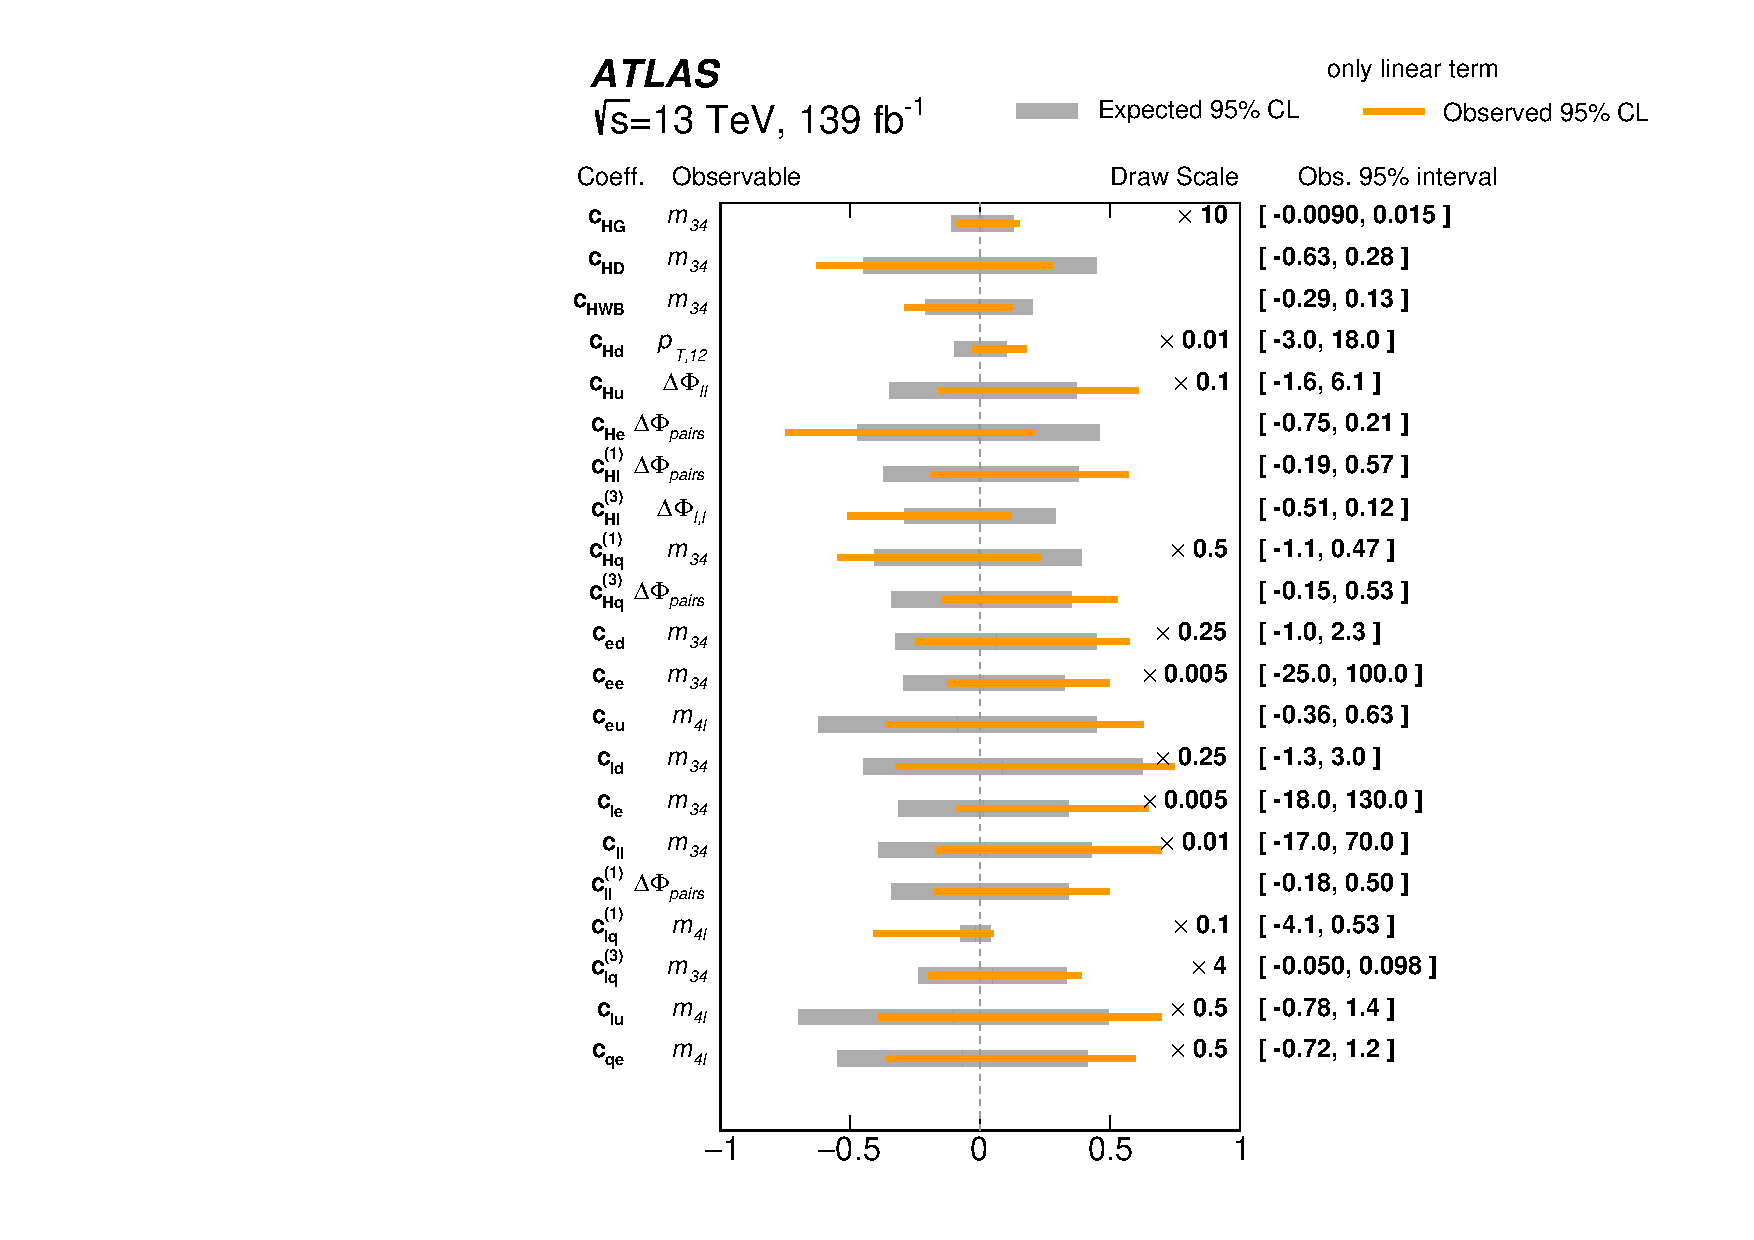
\includegraphics[width=\mediumfigwidth]{Figures/m4l/Interpretations/EFTLimits_linonly_MVozak.pdf}
    \caption{Linear only EFT limits. This figure is from This table is from Ref.~\cite{m4l2021_paper}}
    \label{fig:EFTlinear}
\end{figure} 

\begin{figure}
    \centering
    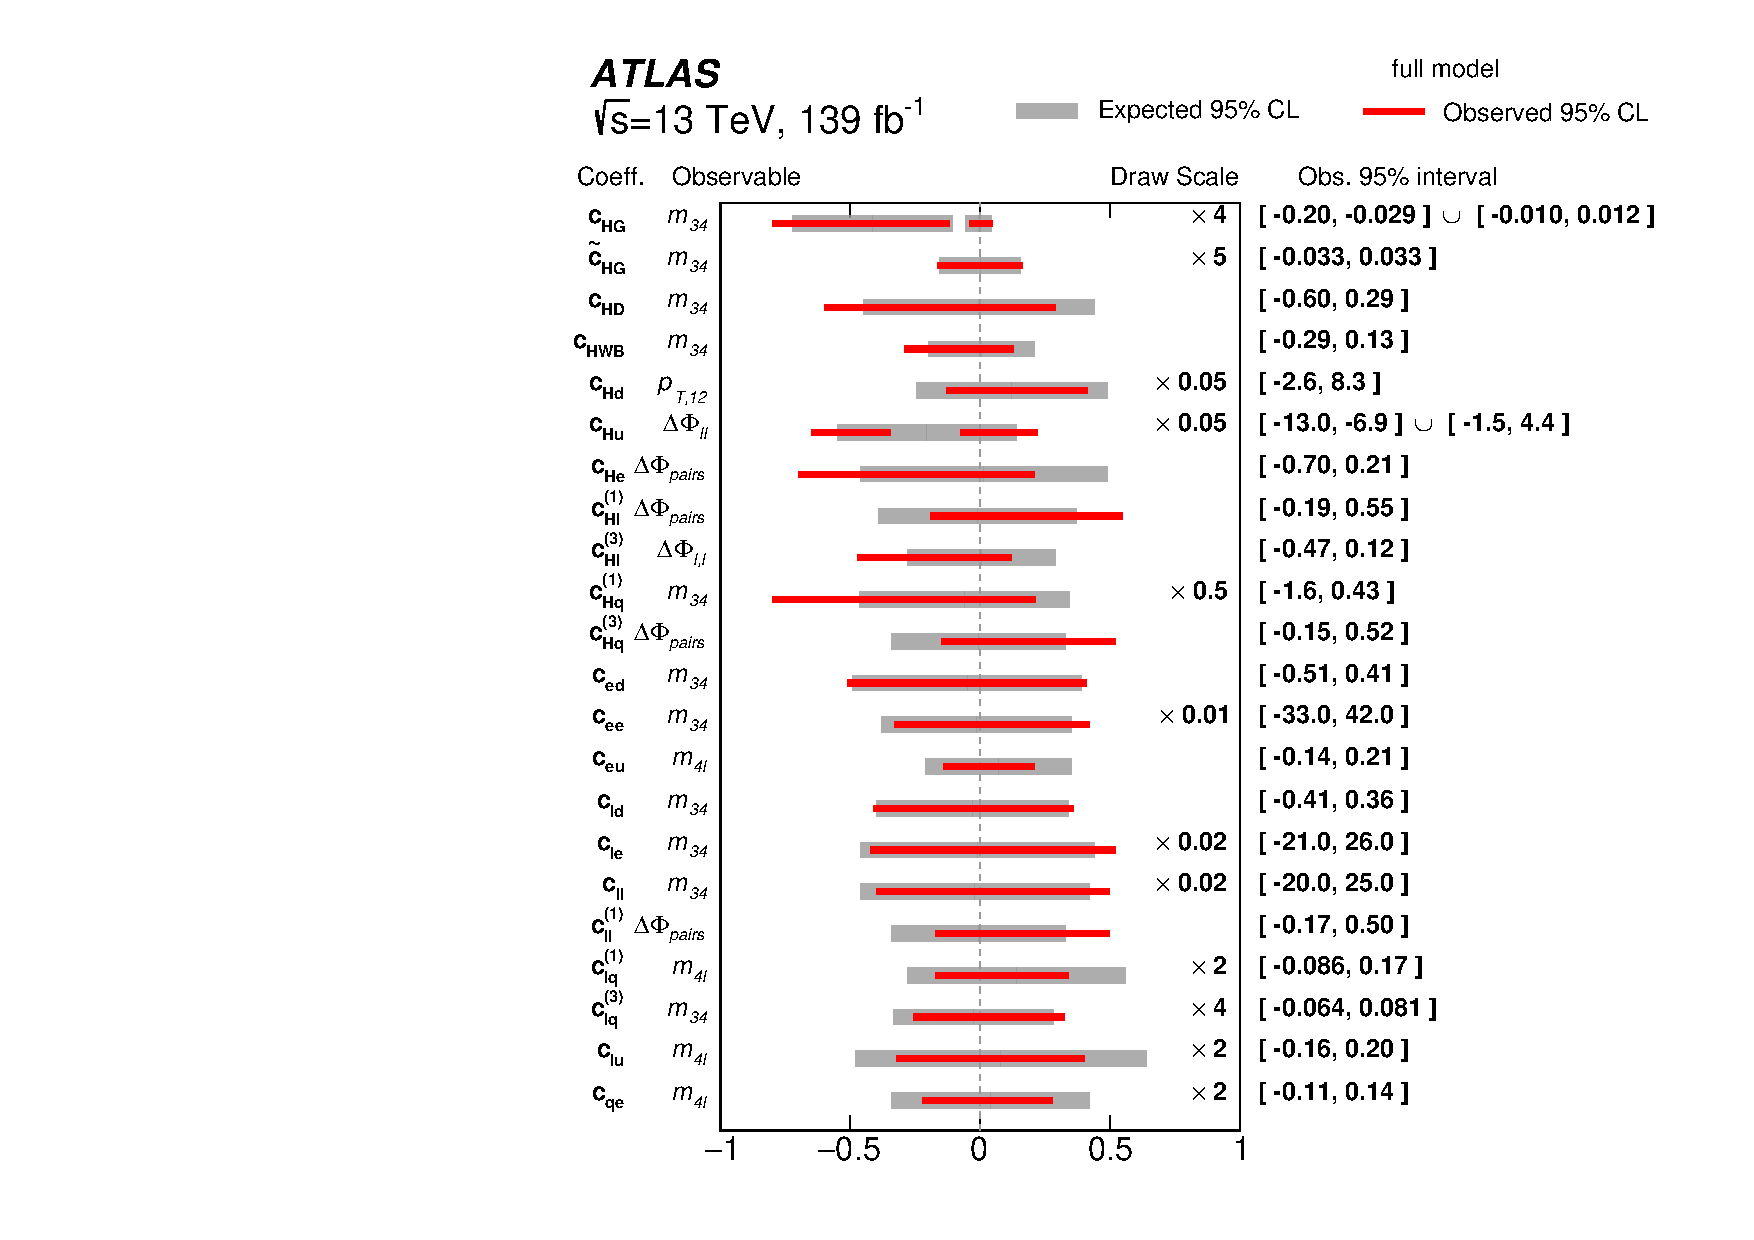
\includegraphics[width=\mediumfigwidth]{Figures/m4l/Interpretations/EFTLimits_MVozak.pdf}
    \caption{Full EFT limits. This figure is from This table is from Ref.~\cite{m4l2021_paper}}
    \label{fig:EFTfull}
\end{figure}

% \subsection{Limits on B-L model}
% \label{ssec:m4l:BL}

% In the theoretical community, several new physics scenarios have been postulated in which the gauge symmetry of the Standard Model are extended via \Ugroup{1} gauge symmetries beyond \Ugroup{1}$_Y$ \cite{}. This class of models is strongly reinforced by the observation of neutrino oscillations, evidence that neutrinos have non-zero mass. They predict three additional SM singlet fermions which are accounted for by right-handed neutrinos, thus enabling the seesaw mechanism of neutrino mass generation. 

% One such model is based on the gauge group \SUgroup{3}$_C\times$\SUgroup{2}$_L\times$\Ugroup{1}$_Y\times$\Ugroup{1}$_{B-L}$, where $B-L$ stands for baryon-number-minus-lepton-number. The \Ugroup{1}$_{B-L}$ symmetry is accompanied by an additional neutral gauge boson $Z'$, an extra SM singlet Higgs $h_2$ which breaks the $B-L$ symmetry, and three generations of right-handed neutrinos. The $Z'$ couples to the SM via $g'$, and the new Higgs $h_2$ mixes with the SM Higgs with mixing angle $\alpha$. The introduction of these new particles may have a non-negligible impact on the phenomenology of the SM, and may manifest themselves in measurements taken at the LHC. 

% A previous study of this model done within the \Contur framework defined five benchmark scenarios using the free parameters of the model. There are six free parameters in total: $M_{Z'}$, $g'$, $M_{h_2}$, $\sin \alpha$, $M_{N_i}$, and $V_{\ell N}$. These correspond to the mass of the new gauge boson and its coupling strength to the SM, the mass of the new Higgs and its mixing angle with the SM Higgs, and the mass  and coupling of the heavy neutrinos. The paper showed that \ATLAS measurements with a four-lepton final state provided significant constraints on certain regions of parameter space. In context of the model, contributions to the spectrum may come from the production of multiple $Z'$, the production of $h_2$ via gluon-gluon fusion which decays via $h_2\rightarrow Z'Z'$ or $h_2\rightarrow ZZ$, or the SM Higgs decaying to a pair of $Z'$. One sensitivity scan published in the study is repeated in this analysis in the plane of the sine of the mixing angle $\alpha$ and the mass of the exotic Higgs boson $m_{h_{\text{2}}}$. The new gauge boson $Z'$ is assumed to have a mass of 35 GeV, and weakly coupled to the SM with $g'=10^{-3}$. 

% The study is presented in Reference~\cite{BLcontur} and a detailed description of \contur can be found in Section~\ref{sec:contur}. In context of this thesis and the \mFourL{} measurement, a further study on the $B-L$ model replicating one benchmark scenario from Reference~\cite{BLcontur} is presented in Chapter~\ref{chap:reinterpretation}.

% An alternate test statistic $\Tilde{q}$ for upper limits is defined using the likelihood function of equation \ref{eq:likelihood} as
% \begin{equation}
%     \tilde{q} = 
%     \begin{cases}
%         - 2 \ln \frac{\mathcal{L}( {\mu}, \hat{\hat{\vec{\theta}}}({\mu})) } {\mathcal{L}(0,         \hat{\hat{\vec{\theta}}}(0) )} & \hat\mu < 0, \\ 
%         - 2 \ln \frac{\mathcal{L}( {\mu}, \hat{\hat{\vec{\theta}}}({\mu})) } {\mathcal{L}(\hat{\mu}, \hat{\vec{\theta}} )} & 0 \leq \hat\mu \leq \mu,  \\ 
%         0 & \hat\mu > \mu.
%     \end{cases}
%     \label{eq:lambda_qtilde}
% \end{equation}
% Here the parameter $\mu$ dictates the strength of the BSM signal process. $\mu = 0$ and $\mu = 1$ correspond to the background-only hypothesis and the nominal signal hypothesis respectively \cite{m4l2021_paper}. The reason for setting $\tilde{q} = 0$ for $\hat{\mu} > \mu$ is that when setting an upper limit, an excess in data (corresponding to large r $\hat{\mu}$) should not be used to reject a signal model with lower yield (lower $\mu$). $\tilde{q}$ is interpreted as an upper
% exclusion limit on the parameter of interest at a certain CL, usually set to 95\%, based on the CLs prescription \cite{CLs_technique} \todo{Maybe say more about p-value to CL?}. 

% The exclusion contour in the plane of $\sin\alpha-m_{h_2}$ is depicted in Figure \ref{fig:BLcontour}, where the variable providing the best expected sensitivity to set the limit. An alternate version using only the inclusive \mFourL distribution to set the limit is shown in Figure \ref{fig:BLcontourm4l}. Corresponding to Figure \ref{fig:BLcontour}, the colour map of Figure~\ref{fig:BLcolourmap} shows the observable used to derive the limits at each point in the parameter space. It is clearly visible that there is a larger excluded region when using the most sensitive observable rather than the \mFourL distribution only. The event kinematics of the BSM model changes as the model parameters change. It is therefore advantageous to exploit various observables accordingly at each model point; ultimately enhancing the sensitivity significantly. This effect is most evident at high $m_{h_2}$, where the expected limit on $\sin\alpha$ strengthens from 0.46 to 0.28. Referring to Figure \ref{fig:BLcolourmap}, the improvements at high $m_{h_2}$ come mainly from the $m_{12}$ distribution. These results demonstrate the power that comes with measuring more variables in regions of phase space. 
% \begin{figure}
%     \centering
%     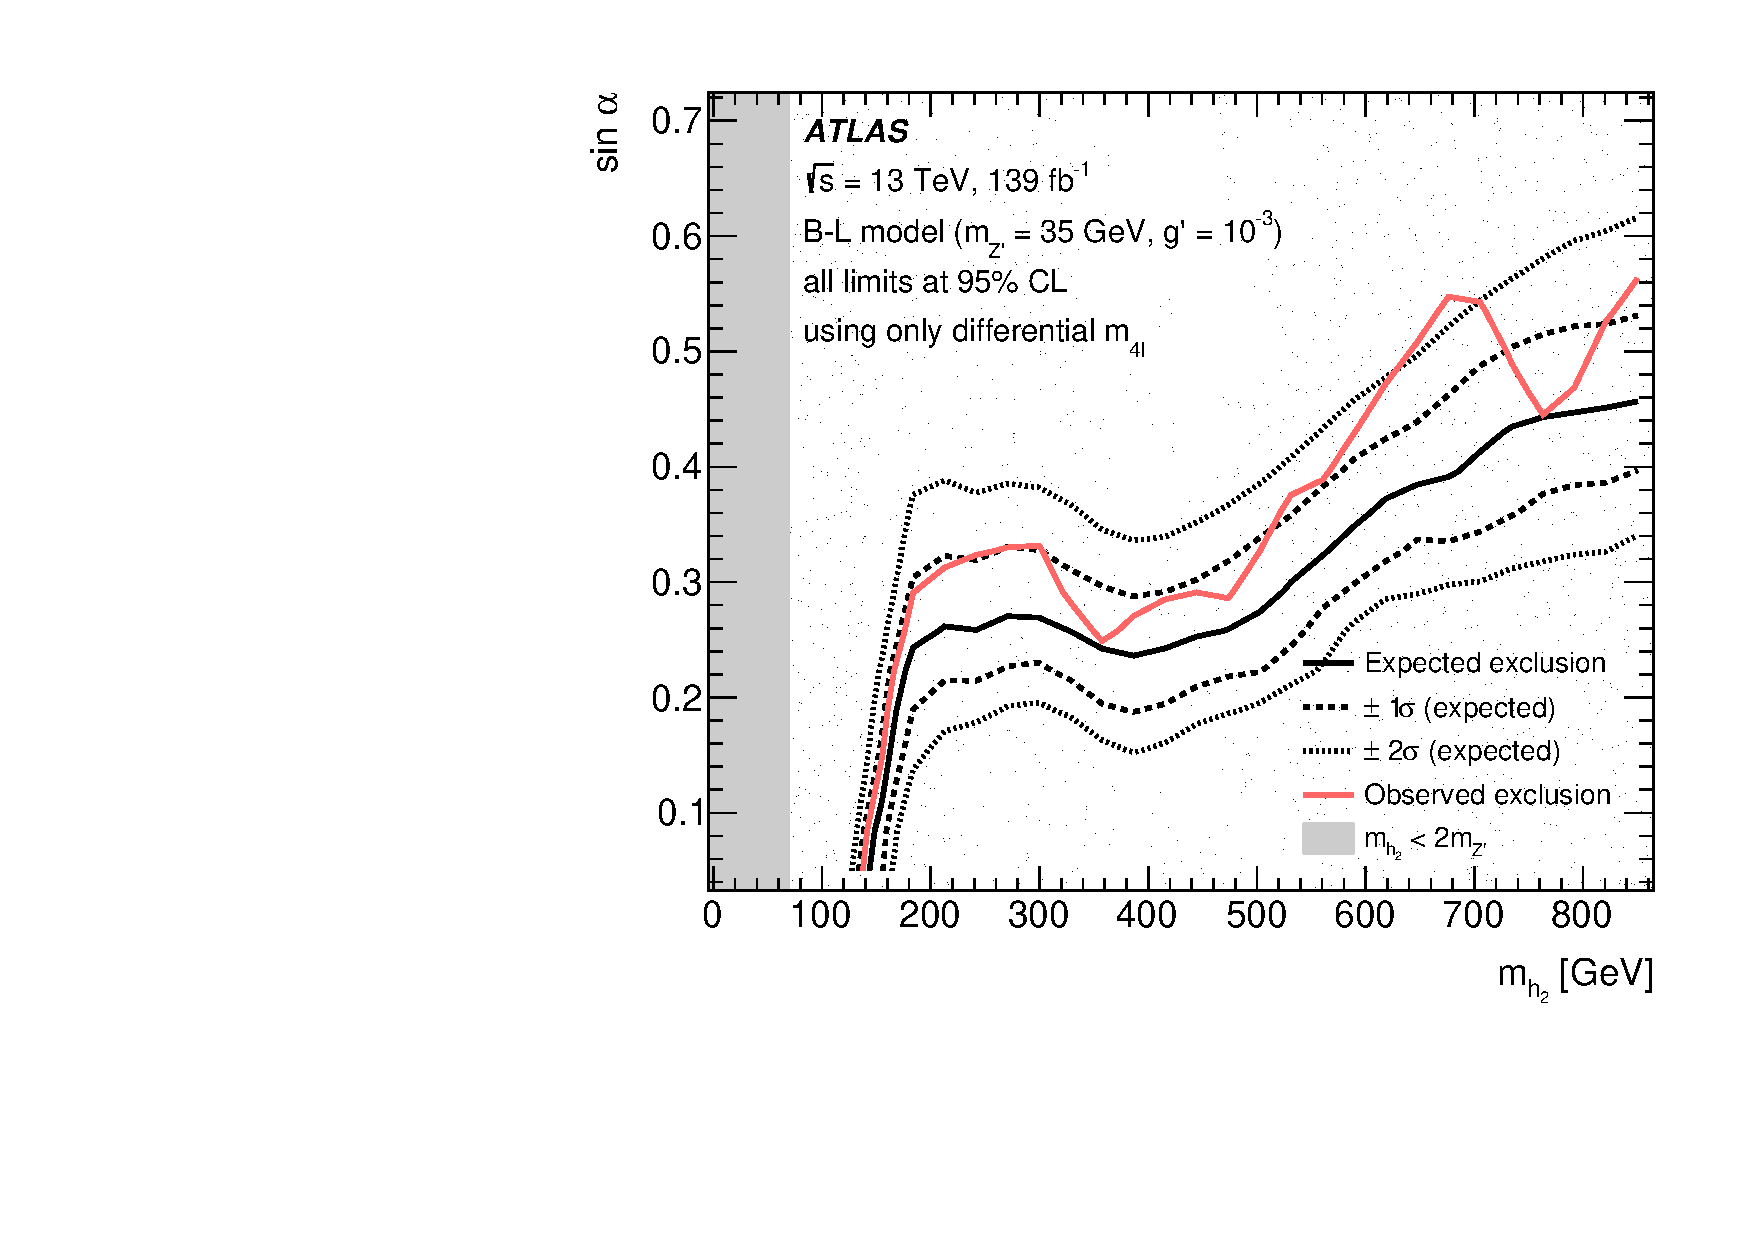
\includegraphics[width=\mediumfigwidth]{Figures/m4l/Interpretations/UpperLimitBandWithContour_2D_withTheoExcl_m4l.pdf}
%     \caption{B-L contour using m4l only}
%     \label{fig:BLcontourm4l}
% \end{figure}
% \begin{figure}
%     \centering
%     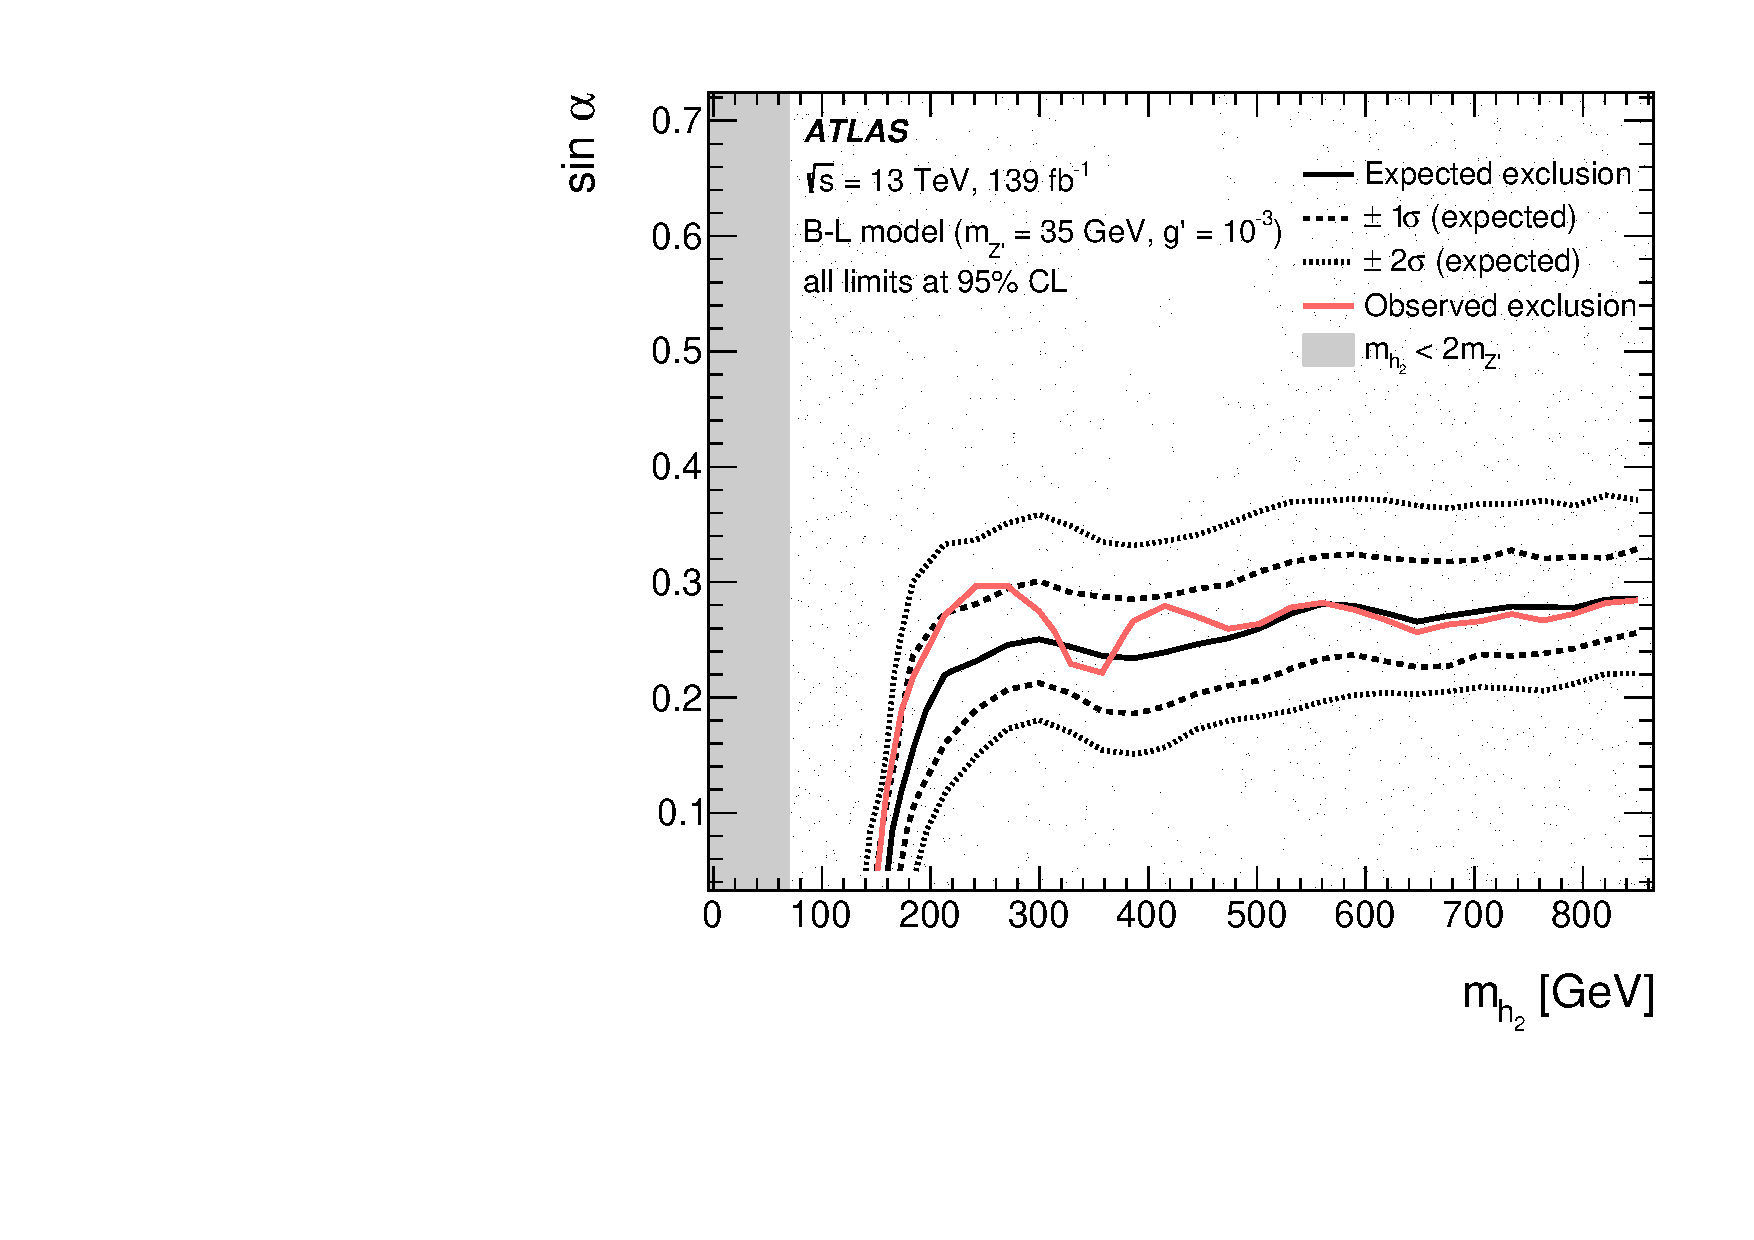
\includegraphics[width=\mediumfigwidth]{Figures/m4l/Interpretations/UpperLimitBandWithContour_2D_withTheoExcl.pdf}
%     \caption{B-L contur using most sensitive variable.}
%     \label{fig:BLcontour}
% \end{figure}
% \begin{figure}
%     \centering
%     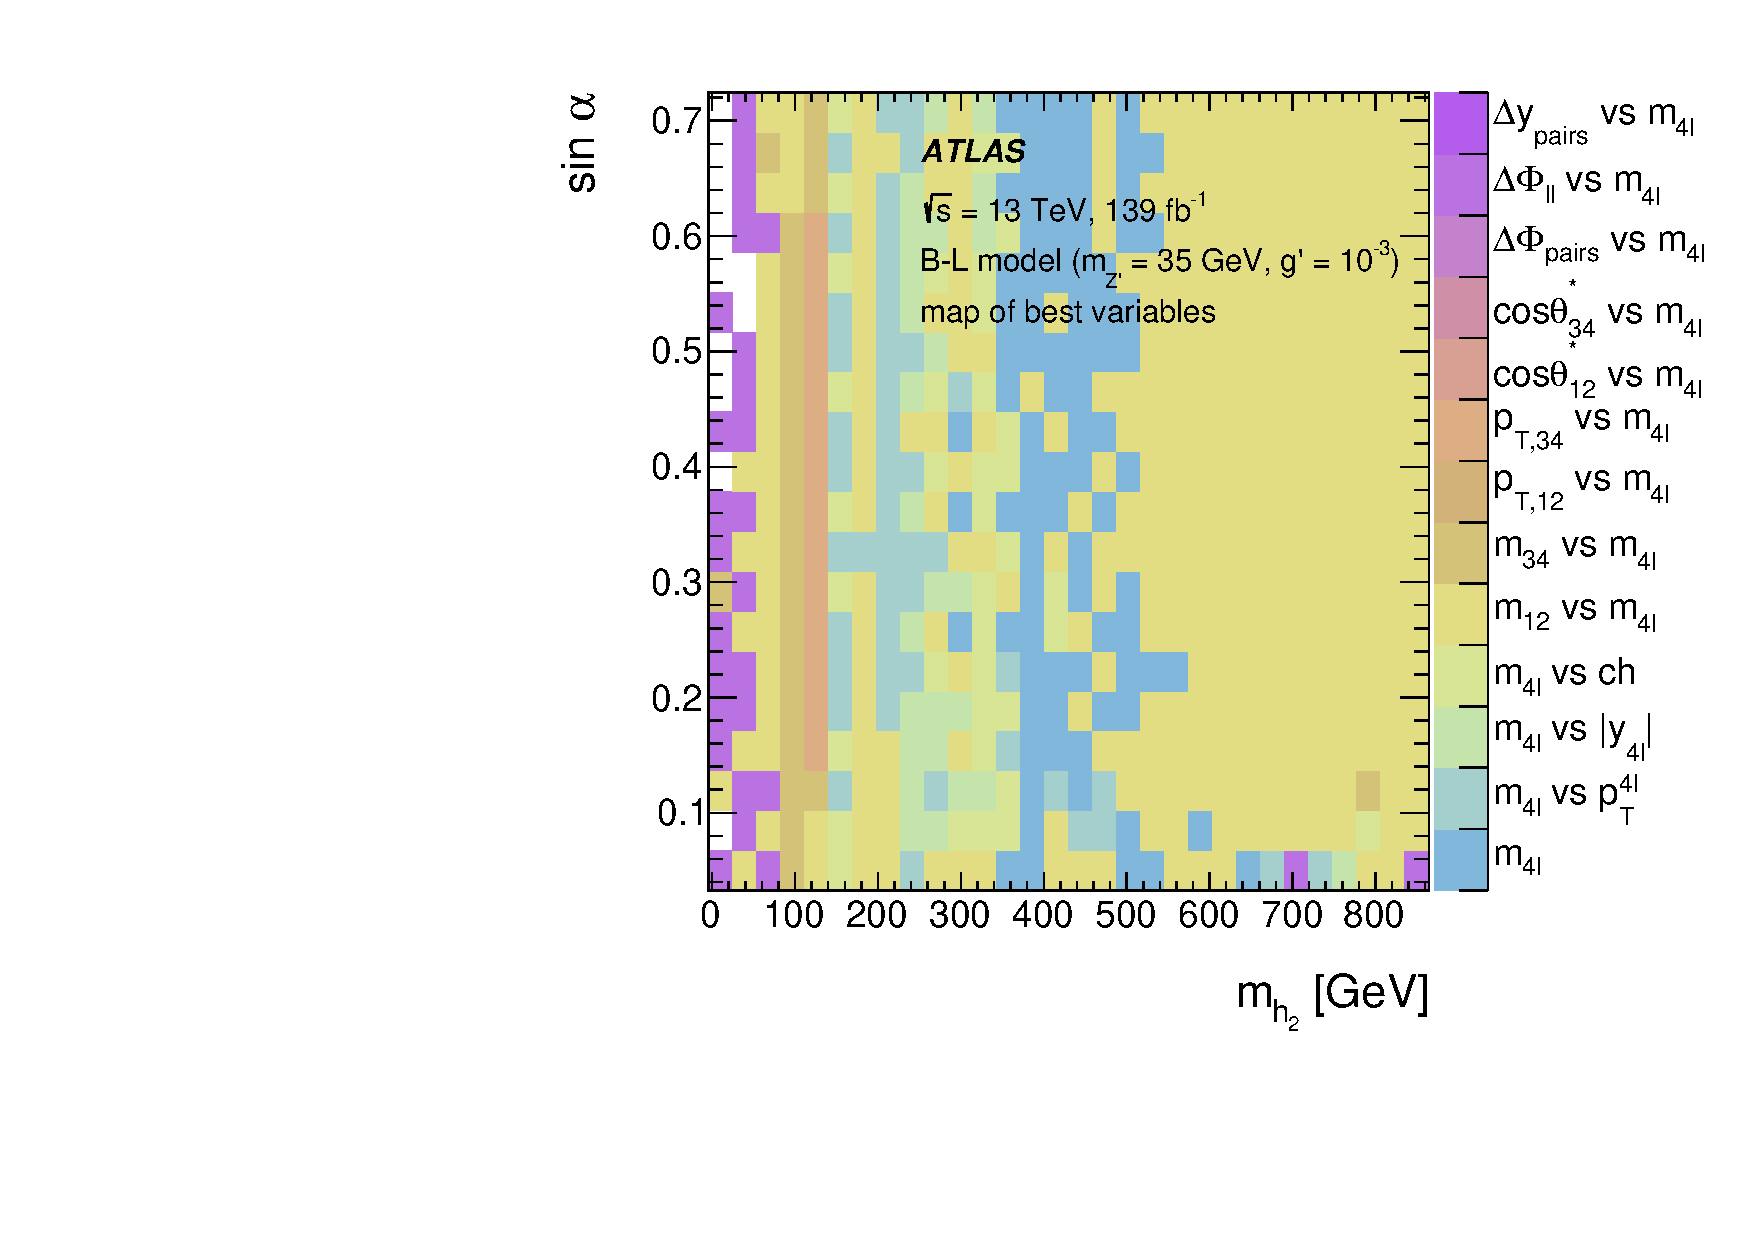
\includegraphics[width=\mediumfigwidth]{Figures/m4l/Interpretations/UpperLimitBandWithContour_2D_colormap.pdf}
%     \caption{B-L colour map}
%     \label{fig:BLcolourmap}
% \end{figure}